\documentclass[conf]{new-aiaa}
%\documentclass[journal]{new-aiaa} for journal papers
\usepackage[utf8]{inputenc}

\usepackage{amsmath}
%\usepackage{amsthm}
%\usepackage{amssymb}
\usepackage{graphicx}
\usepackage{float}
\usepackage{listings}
\usepackage{caption}
\usepackage{subcaption}
\bibliographystyle{new-aiaa}

\usepackage{multicol}
%\usepackage{bm}
%\usepackage{physics}



%%%%%%%%%%%%%%%%%%%%%%%%%%%%%%%%%%%%%%%%%%%%%%%%
%
%  This is all the stuff for Python code snippets
%
\DeclareFixedFont{\ttb}{T1}{txtt}{bx}{n}{10} % for bold
\DeclareFixedFont{\ttm}{T1}{txtt}{m}{n}{10}  % for normal
% Custom colors
\usepackage{color}
\definecolor{deepblue}{rgb}{0,0,0.5}
\definecolor{deepred}{rgb}{0.6,0,0}
\definecolor{deepgreen}{rgb}{0,0.5,0}

\setcounter{MaxMatrixCols}{15}

% Python style for highlighting
\newcommand\pythonstyle{\lstset{
		language=Python,
		basicstyle=\ttm,
		morekeywords={self},              % Add keywords here
		keywordstyle=\ttb\color{deepblue},
		emph={MyClass,__init__},          % Custom highlighting
		emphstyle=\ttb\color{deepred},    % Custom highlighting style
		stringstyle=\color{deepgreen},
		frame=tb,                         % Any extra options here
		showstringspaces=false,
		tabsize=4
}}

% Python environment
\lstnewenvironment{python}[1][]
{
	\pythonstyle
	\lstset{#1}
}
{}

% Python for inline
\newcommand\pythoninline[1]{{\pythonstyle\lstinline!#1!}}

%%%%%%%%%%%%%%%%%%%%%%%%%%%%%%%%%%%%%%%%%%%%%%%%%


\newcommand{\mpc}{MPC}
\newcommand{\nmpc}{NMPC}
\newcommand{\pdiff}{P_{\Delta}}
\newcommand{\pavg}{\overline{P}}
\newcommand{\R}{\mathbb{R}}
\newcommand{\casadi}{CasADi}
\newcommand{\dompc}{{\bf do-mpc}}

\title{Comparison of Direct Methods for NMPC Applied to a Thrust-Vector-Controlled Drone}
\author{Isidore Mones and Heidi Dixon}
%\date{}

\begin{document}
\maketitle
\renewcommand{\thefootnote}{\arabic{footnote}}
\begin{abstract}
 
We developed a nonlinear model predictive control (NMPC) framework for a thrust vector control (TVC) drone. Designed to study vertical takeoff and landing (VTOL), the drone has a two-axis gimbal and two stacked counter-rotating brushless motors for thrust.
The drone's control loop runs at 50 Hz on the Raspberry Pi 5, so computational efficiency is important.
The primary computational task of an NMPC solver is the solution of the embedded nonlinear programming problem (NLP).
We experimented with three formulations for the NLP:  a standard multiple shooting version, a Chebyshev pseudospectral collocation method, and an orthogonal collocation method.  
The methods are compared on three simulation test cases with varying initial conditions and difficulty. Performance metrics included average CPU time, maximum CPU time, the number of NLP solver failures, settling time, and trajectory smoothness.
All methods had average solution times below the required $0.02s$ time threshold and would likely provide viable solutions for NMPC on the drone. 
Orthogonal collocation demonstrated the most reliable performance, meeting the timing constraints for all NLP solver calls while producing smooth convergent trajectories without NLP solver failures. Initial hardware experiments using orthogonal collocation showed successful closed-loop hover stabilization on the physical drone.


\end{abstract}
\section{Introduction}	
	
	This paper is inspired by the gimballed-thrust drone prototype developed by Linsen et al. \cite{TVCDrone}.
	The value of propulsive VTOL with TVC is illustrated by VTOL milestones like NASA's Lunar Landing Research Vehicle (LLRV) which allowed Apollo astronauts to practice lunar landings, McDonnell Douglas’s DC-X (Delta Clipper), and SpaceX's Falcon 9 and Starship landings, the latter to be used in the planned Artemis IV mission that aims to land and return astronauts from the moon.	

	Near the upright hover equilibrium, vertically flying rockets are open-loop unstable in attitude. They have highly nonlinear, coupled dynamics, and require fast control algorithms that respond quickly to disturbances and sensor noise. Unfortunately, validating control techniques on full-scale rockets is prohibitively costly and high-risk. There is a need for inexpensive test vehicles that allow experimentation with rocket guidance, navigation, and control. 

	A gimballed-thrust drone with electric motors and propellers is a good choice for replicating rocket dynamics on a much smaller budget. A couple of low-cost designs have been proposed and implemented  \citep{cheapTVC}, \citep{TVCDrone}. The drone design by \cite{TVCDrone} allows experimentation with control algorithms for VTOL and TVC. We have designed a similar drone based on their images and design descriptions, and there remain many details and design choices to explore.



	Our drone implements TVC and VTOL using a nonlinear model predictive control (NMPC) algorithm, allowing it to handle nonlinear rocket dynamics and manage constraints like gimbal angle range, servo rates, and thrust limits. NMPC optimizes control inputs across a finite time horizon at each time step. In this sense, it optimizes a control sequence, allowing it to anticipate future control requirements. Revising the sequence at each time step allows it to respond to disturbances. The main downside of NMPC is its high computational load. NMPC solves a constrained Optimal Control Problem (OCP) that is transcribed into a finite dimensional nonlinear programming problem (NLP) at every control step, and as a result it is much slower than simple control algorithms like proportional-integral-derivative (PID) controllers or linear quadratic regulators (LQR).



	There are a variety of ways to formulate NMPC problem instances as NLPs. Different formulations  vary in their computation times and solution accuracy, particularly on embedded hardware platforms with limited computational resources.
	In this paper we focus on evaluating different NLP formulations. We  compare three approaches: a Runge-Kutta multiple shooting method, an orthogonal collocation  implemented in the {\bf do-mpc}  library \citep{do-mpc},  and a Chebyshev pseudospectral collocation approach. 
	Simulations are run on a Raspberry Pi 5 at $50$ Hz, so solution speed is a very important consideration.
	Methods are compared on the basis of computational performance, numerical reliability, and trajectory quality in a set of simulated flight scenarios.  


	This paper is structured as follows.  Section \ref{hardware} covers drone hardware components and design, the mathematical model is described in section \ref{equations}. Sections \ref{nmpc} and \ref{nlp} cover the NMPC algorithm and NLP formulations. Experimental results are presented in section \ref{results} and section \ref{hardwarevalidation} covers future work. We finish with conclusions in section \ref{conclusion}.
	Code for this project is available at the GitHub repository https://github.com/izzymones/hop
	
\section{Hardware Design}
\label{hardware}
The vehicle design is inspired by the EPFL thrust-vectoring research drone \cite{TVCDrone}, with an emphasis on repairability, ease of modification, and compatibility with common off-the-shelf flight hardware.
Our drone has a total mass of 1.5 kg, with a diameter and height of 260mm and 500 mm respectively. It is powered by a 6S battery.
The propellers are collinear and counter-rotating to allow for yaw controllability. They are driven by BrotherHobby 2207 BLDC motors. 
The vehicle center of mass is located near the central body axis, with its exact position determined primarily by the placement of the battery, onboard computer, flight controller, and power electronics. The thrust vector angles are  actuated using a two-axis gimbal with PDI-6621MG servos.
The drone uses the Pixhawk onboard IMU, barometer, and magnetometer, along with an M9N GPS for outdoor positioning and an ARK Flow optical-flow sensor for indoor or GPS-denied flight. 
State estimation is performed using the Pixhawk’s onboard Extended Kalman Filter, which fuses measurements from the onboard IMU, barometer, magnetometer, GPS, and optical-flow sensor.

Onboard computation is split between a Raspberry Pi 5 and a Pixhawk 4 flight controller. The Raspberry Pi 5 runs the nonlinear model predictive controller, while the Pixhawk 4 handles sensor fusion and actuator command passthrough. 
Communication between the controller on the Raspberry Pi and the Pixhawk is handled through ROS 2 running on Ubuntu 24.04 LTS. The Raspberry Pi sends actuator commands to the Pixhawk, and receives state estimates from it. This architecture allows the computationally expensive control algorithm to run on the Raspberry Pi while preserving the Pixhawk’s robust sensor fusion and hardware interfacing capabilities.

\begin{figure}
	\centering
	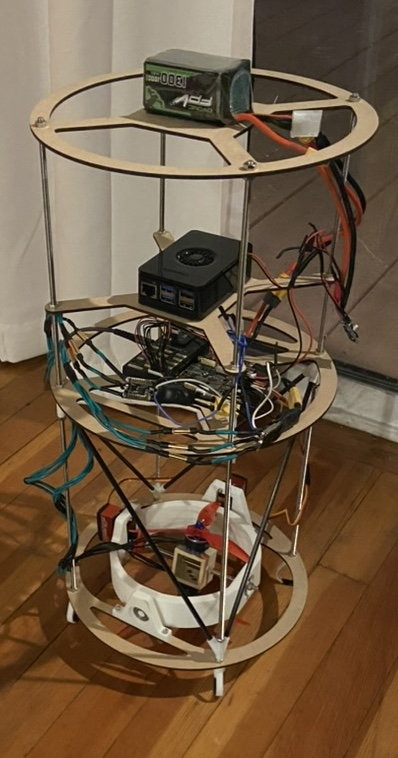
\includegraphics[width=0.3 \textwidth]{figures/dronePic.jpeg}
	\caption{TVC Drone Prototype}
	\label{fig:dronePic}
\end{figure}


\section{Equations of Motion}
\label{equations}

The system state $\vec{x}$ includes translational position $\vec{p} = [x, y,  z]$ in meters and velocity $\vec{v} = [v_x, v_y, v_z ]$ in meters per second both expressed in the world frame. The attitude is represented as a unit quaternion $\vec{q} = [q_x, q_y,  q_z, q_w]$. The angular velocity in the body frame $ \vec{\omega} = [\omega_x, \omega_y, \omega_z]$ is in radians per second yielding the full state vector $\vec{x} = [\vec{p}, \vec{v}, \vec{q},  \vec{\omega} ]$. The control vector $\vec{u} =[ \theta_1, \theta_2, \pavg, \pdiff ]$ includes the two gimbal angles $\theta_1, \theta_2 $ in degrees, the average thrust between the two propellers, $\pavg$, with values from $[0, 1]$, and the differential thrust between the propellers $\pdiff$ which  controls the rotation about the body $z$ axis and takes values in $[-1, 1]$.

The equations of motion are represented as the standard 6DOF series of first-order vector differential equations:
\begin{gather}
	\dot{\vec{p}}  = \vec{v}         \label{eqMotion1}	\\
	\dot{\vec{v}}  = \frac{1}{m}R(\vec{q})\vec{F_b}+\vec{g}  \label{eqMotion2} \\
	\dot{\vec{q}} = \frac{1}{2}Q(\vec{\omega})\vec{q}  \label{eqMotion3} \\
	\dot{\vec{\omega}} = I^{-1}\!\left(\vec{M_b} - \vec{\omega} \times (I\,\vec{\omega})\right) \label{eqMotion4}
\end{gather}
where $m$ is the mass of the drone and $\vec{g} = [0, 0, -9.81]^T$ is the acceleration due to gravity. The body to world rotation matrix $R(\vec{q})$  is used to compute the force in world coordinates due to the body-centric thrust vector given the quaternion orientation. Using vector decomposition we can find the thrust vector in body coordinates $\vec{F_b}$ in terms of the gimbal angles $\theta_1$ and $\theta_2$ and magnitude of the thrust $T$ acting on the drone. The gimbal angles  are commanded in degrees but converted to radians in the dynamics model.

\[
\vec{F_b} = T
\begin{bmatrix}
	\sin{\theta_{2,\text{rad}}}  \\
	-\sin{\theta_{1,\text{rad}}}\cos{\theta_{2,\text{rad}}}  \\
	\cos{\theta_{1,\text{rad}}}\cos{\theta_{2,\text{rad}}}
\end{bmatrix}
\]
The quaternion propagation matrix $Q(\vec{\omega})$ computes the change in quaternions given a set of angular velocities.
The inertia tensor $I$ is computed from a CAD model of the drone.
The body frame moment vector $\vec{M_b}$ is the sum of the torque due to thrust vector $\vec{F_b}$ acting through the moment arm $ \vec{l} = [0, 0, -l]^T$ and the torque generated about the body $z$ axis by the differential thrust $ \vec{M_z} = [0,0, M_z]^T$. 
\[
\vec{M_b} = \vec{l} \times \vec{F_b} + \vec{M_z}=       
\begin{bmatrix}
	-lT\sin{\theta_1}\cos{\theta_2}  \\
	-lT\sin{\theta_2}  \\
	M_z
\end{bmatrix}
\]
The value $l$ is the moment-arm length from the center of mass to the point where $\vec{F_b}$ acts on the drone in body coordinates. 

Note that these equations use the variable $T$ representing the magnitude of the thrust vector acting on the drone. 
The actual control variables are defined as the average $\pavg=\frac{T_1+T_2}{2}$ and difference $\pdiff = T_1-T_2$ between the two stacked propeller thrust values $T_1$ and $T_2$. The command signals for motors $T_1$ and $T_2$ take values in $[0,1]$. 
To map the average thrust command signal value to the actual thrust force value in Newtons, a second-order polynomial fit is experimentally determined
\[
T = a\Big(\pavg  \frac{v}{25}\Big)^2+b\Big(\pavg \frac{v}{25}\Big)+c
\]
where $v$ is the current voltage of the 25V battery. Similarly, a linear relationship is used to map the differential thrust to the moment about the body frame $z$ axis.
\[
M_z = d I_{zz} \pdiff
\]





	\section{Nonlinear Model Predictive Control (NMPC)}
	\label{nmpc}
Model predictive control (\mpc)  \cite{mpc} is a control algorithm that solves an optimization problem at each time step. It returns a series of control inputs over a finite time horizon, creating a {\em plan} of actions that can anticipate and adjust to future issues. The control values for the first step of the plan are applied to the system and then the plan is revised at the next time step, allowing the system to respond to disturbances and noise. The {\mpc} framework also allows us to enforce the mechanical limitations of our thrust motors and gimbal servos. Nonlinear model predictive control (\nmpc) is a variant of {\mpc} that can handle nonlinear dynamics.   Working directly with the nonlinear equations allows more accurate predictions of the drone behavior.  Libraries like {\casadi} \cite{casadi} and {\dompc} \cite{do-mpc} make {\nmpc} NMPC more accessible in practice.

An {\nmpc} instance for the thrust vector drone is a minimization problem of the form
\begin{align}
	\min_{u(t)} \; &  \int_{0}^{t_f} \ell(x(t),u(t))\,dt  \;+\; \phi(x_f) \nonumber \\
	\text{s.t.} \;\; 	&  \dot{x} =  f(x(t),u(t))  \nonumber \\ 
	& x(0) = x_0 \nonumber \\
	&	-\theta_{max} \leq \theta_1 \leq \theta_{max} \nonumber \\
	& 	-\theta_{max} \leq \theta_2 \leq \theta_{max} \nonumber \\
	& 	T_{min}  \leq \pavg + \pdiff/2 \leq T_{max} \nonumber  \\
	&    T_{min} \leq  \pavg - \pdiff/2 \leq T_{max} \nonumber \\
	%	&       T_{diff_{min}} \leq \pdiff \leq T_{diff_{max}} \label{nmpc:thrust3} \\
	& 	-\dot{\theta}_{max} \leq \dot{\theta}_1 \leq \dot{\theta}_{max} \nonumber \\
	&  	-\dot{\theta}_{max} \leq \dot{\theta}_2 \leq \dot{\theta}_{max} \nonumber \\ 
	&        0 \leq z.\nonumber
\end{align}
The problem instance enforces minimum and maximum gimbal angles of $\pm 20^{\circ}$ for the outer gimbal and $\pm 13.5^{\circ}$ for the inner gimbal, minimum and maximum thrust ranges, rate constraints for the servos and restrictions on the drone's vertical height.

The cost function  minimizes both the squared error between the current state $x(t)$ and the goal state $x_{r}$ weighted by diagonal matrix $Q$ and the error between the current control $u(t)$ and the goal control $u_{r}$ weighted by diagonal matrix $R$. 
\begin{equation*}
	\ell(x(t),u(t))= (x(t)-x_{r})^T Q (x(t)-x_{r}) + (u(t)-u_{r})^T R (u(t)-u_{r}) 
\end{equation*}
The terminal cost  
\begin{equation*}
	\phi(x_f) = (x(t_f)-x_{r})^T Q_f (x(t_f)-x_{r})
\end{equation*}
prioritizes solutions with the final state in the horizon close  to the goal state.



\section{NLP Formulations}
	\label{nlp}
	To solve the continuous time optimal {\nmpc} instance, it is formulated as a discrete time finite dimensional nonlinear programming problem (NLP) and solved by a standard NLP solver.  
	Since the system was intended as  a real-world TVC drone prototype, a major design consideration was implementation simplicity. Multiple shooting and orthogonal collocation methods met these criteria, multiple shooting because it is easy to understand, and orthogonal collocation because it is available through  the {\dompc} Python toolbox \cite{do-mpc}. Chebyshev pseudospectral collocation is more challenging to implement, but it has been used successfully before for a TVC drone \cite{TVCDrone} suggesting it could meet the computational requirements. For each method we ran tuning experiments to select the optimal parameters for the method. All tuning experiments were run on the Raspberry Pi 5 with a 2.4 GHz CPU and 8GB RAM running Ubuntu 24.04 LTS. To solve our nonlinear programming (NLP) problems we used the \texttt{ipopt} solver \cite{ipopt} that comes installed with CasADi 3.7.1 \cite{casadi}.   This solver requires an additional subroutine to  solve sparse matrix systems. After some experimentation we chose to use the \texttt{ma27}  solver  from HSL (Harwell Subroutine Library) \cite{hsl}. 	We implemented warm starts for all of our methods by seeding the initial guess for the NLP with the state and control values from the previous time step. All methods used a one second prediction horizon.
	
	In multiple shooting \cite{multipleShootingCanon, multipleShootingpractical}, we divide our prediction horizon into $N$ evenly spaced intervals of length $\Delta t$ defined by nodes $\{ t_0, t_1, \ldots, t_N \}$ and we make copies of our state $x_k$ and control $u_k$ variables for each time step.  The initial state is initialized to the current state. 	Using the system dynamics $\dot{x} =  f(x(t),u(t))$ and Runge-Kutta 4 within each time step $[t_k, t_{k+1}]$ we forward integrate our differential equations to create constraints that enforce the change of state between time steps. 
	We built our multiple shooting formulation in Python with CasADi 3.7.1 \cite{casadi}.  Tuning experiments across a range of test cases showed that $N=4$ time intervals across the 1 second prediction horizon provided the best smoothing and settling scores while still meeting timing criteria.
	
	
	 Orthogonal collocation on finite elements with Gauss-Radau nodes as implemented in {\dompc}, allows rapid development and testing of embedded NMPC controllers with minimal implementation overhead. 
	The prediction horizon is divided into $N$ time intervals of equal duration called finite elements. 
	Within each finite element, the differential equations $\dot{x} =  f(x(t),u(t))$ are approximated with a polynomial of order $K+1$ and interpolated over $j = 0, 1, \ldots, K$ interpolation points within the interval.
	Continuity constraints are added at the boundaries of adjacent finite elements to ensure continuity of the state trajectory. Implementation details for {\dompc}'s orthogonal collocation method can be found in the work of Biegler  \cite{dompc-oc}.  Tuning experiments across a range of test cases showed that $N=4$ time intervals across the 1 second prediction horizon with $K=2$ provided the best smoothing and settling scores while still meeting timing criteria.

	Chebyshev pseudospectral methods approximate the state and control trajectories using global high-order polynomials over the prediction horizon. Dynamics are enforced at Chebyshev collocation points, which are distributed non-uniformly to reduce interpolation error that can occur near interval endpoints. This allows the method to accurately enforce the system equations with fewer collocation points. Our implementation is based on the work of Fahroo et. al.  \cite{chebyshevPS} and was implemented with CasADi 3.7.1 \cite{casadi}.  The solution of the NLP for this method often failed to converge within the allotted number of NLP iterations. Increasing the number of collocation points didn't lead to noticeably better performance. 
	Removing the servo rate constraints reduced this problem so we leave those constraints  out in our comparison with the other methods. After running multiple test cases we found that $6$ collocation points were required to produce adequate smoothness and settling times within the required time limits.
	

	

	
\section{Results}
\label{results}

	To compare the performance of the three NLP formulations, we ran simulations on three test cases with different levels of perturbation from the goal state.
	All test cases used a goal state with the position $\vec{p} = [0, 0,  0]$, a vertical orientation and no translational or angular velocity.
	The first case begins in the goal state and must simply hover to maintain the goal state. The second test state begins at  position of $\vec{p} = [1, 1, 0]$ and must move to the goal state. The third begins at a position $\vec{p} = [1, 0.5, 1]$, has a $15^{\circ}$ tilt from vertical, a slight rotation around the $z$ axis and some velocity in both the $x$ and $y$ directions.

	For each simulation, the following metrics were evaluated: average CPU time, worst-case CPU time, number of NLP solver failures, settling time, and smoothness of the resulting state and control trajectories.
	NLP failures are defined as any solver termination that did not return the \texttt{ipopt} status \texttt{SolverSucceeded}. This happens when the solver exceeds the maximum iteration count, fails to converge, or is given an infeasible problem.
	When evaluating NMPC performance, computational efficiency needs to be balanced against trajectory quality. In particular, trajectories should converge promptly to the goal state while maintaining smooth state and control trajectories. 
	For a trajectory with $N$ time steps, the smoothness metric $S$ was defined as
\[
S
=
\sum_{k=1}^{N-1}
\left\|
\vec{x}_{k+1} - \vec{x}_k
\right\|^2
\]
	with lower values of $S$ corresponding to smoother trajectories.
	Settling time was defined as the first time the system state enters and remains within a specified tolerance region around the goal state:
\[
t_s
=
\min \left\{
t_k :
\|\vec{e}_j\| < \epsilon,
\ \forall j \ge k
\right\}
\]
	All simulations were executed on a Raspberry Pi 5 with a 2.4 GHz CPU and 8 GB RAM running Ubuntu 24.04 LTS. The control loop operated at 50 Hz, corresponding to a real-time control interval of $0.02$s. The equations of motion were forward propagated using a fourth-order Runge--Kutta integrator at 200 Hz.

	Tables (\ref{table1}), (\ref{table2}), and (\ref{table3}) summarize the performance metrics for all three test cases. NLP solver failures occurred only in the multiple shooting formulation and were infrequent.
	All three methods achieved similar average CPU times, and the average solve time remained below the $0.02$s real-time threshold in all test cases. However, the worst-case solve times for both multiple shooting and Chebyshev pseudospectral collocation exceeded the real-time limit in some cases. The timing plots in Figure (\ref{fig:timingplots}) show that Chebyshev pseudospectral collocation exceeded or came close to the threshold frequently, whereas multiple shooting exceeded the threshold only twice. Orthogonal collocation was the only formulation that remained within the time constraint for every NMPC solve.
	Settling times were similar across all methods and test cases, as shown in Tables (\ref{table1}), (\ref{table2}), and (\ref{table3}) and in the state trajectories of Figures (\ref{fig:state1}), (\ref{fig:state2}), and (\ref{fig:state3}). State trajectory smoothness metrics were also low across all methods, indicating smooth convergence behavior.
	The Chebyshev pseudospectral collocation method produced higher control trajectory smoothness scores overall, particularly in test cases two and three, indicating less smooth control inputs than the other formulations. This might be caused by the removal of servo rate constraints that was needed to avoid NLP failures during tuning.


	While all three NLP formulations appear feasible for implementation on the proposed drone platform, orthogonal collocation was selected for the final controller implementation. Compared with the other formulations, orthogonal collocation provided the most consistent real-time performance, with worst-case solve times remaining below the $0.02$s control interval for all test cases. In addition, it exhibited no NLP solver failures and produced smooth state and control trajectories with rapid convergence to the goal state. These characteristics make orthogonal collocation the most reliable formulation for real-time deployment on the Raspberry Pi 5 based flight controller.
		

	
	\begin{table}[ht]
		\centering
		\begin{subtable}[b]{0.5\textwidth}
			\centering
			\begin{tabular}{ | l | c | c | c | } 
				\hline
				& OC & CPS & MS  \\
				\hline
				average CPU (sec) &            0.012        &        0.013         &        0.01  \\ 
				worst case CPU (sec)  &    0.014           &     0.025             &   0.061    \\  
				NLP failures &     0        &            0               &     1  \\
				settle time   (sec) &       2.62          &       2.14       &          2.46  \\ 
				state smoothness &        0.004        &        0.003   &             0.002   \\
				control smoothness &       0.08          &      0.314      &          0.028   \\
				\hline
			\end{tabular}
			\caption{Hover}
			\label{table1}
		\end{subtable}
		\hfill
		\begin{subtable}[b]{0.5\textwidth}
			\centering
			\begin{tabular}{ | l | c | c | c | } 
				\hline
				& OC & CPS & MS  \\
				\hline
				average CPU (sec) &           0.01         &       0.009      &          0.009  \\ 
				worst case CPU (sec)  &  0.013           &     0.015         &       0.045    \\  
				NLP failures &     0         &           0           &         1   \\
				settle time   (sec) &      3.64       &          3.06        &         3.44   \\ 
				state smoothness &      0.211       &         0.269       &         0.076 \\
				control smoothness &   4.697       &        35.606     &           0.878   \\
				\hline
			\end{tabular}
			\caption{Initial position of $[1, 1, 0]$}
			\label{table2}
		\end{subtable}
		\hfill
		\begin{subtable}[b]{0.5\textwidth}
			\centering
			\begin{tabular}{ | l | c | c | c | } 
				\hline
				& OC & CPS & MS  \\
				\hline
				average CPU (sec) &           0.01       &         0.008        &        0.009   \\ 
				worst case CPU (sec)  &    0.015      &           0.013        &        0.012  \\  
				NLP failures &   0        &            0           &         0 \\
				settle time   (sec) &       5.52     &            6.24       &          6.98  \\ 
				state smoothness &      0.939      &          0.919       &         0.738  \\
				control smoothness &     43.011    &          330.531      &          4.534   \\
				\hline
			\end{tabular}
			\caption{Initial position $\vec{p} = [1, 0.5, 1]$, $15^{\circ}$ tilt, $10^{\circ}$ about $z$,  $+v_x$, $+v_y$ }
			\label{table3}
		\end{subtable}
		\caption{Performance metrics for three test cases}
		\label{tables}
	\end{table}


 %-------------------------------------- HOVER EXAMPLE ------------------------------------------
 
 \begin{figure}[H]
 	\centering
 	 \begin{subfigure}[b]{0.3\textwidth}
 		\centering
 		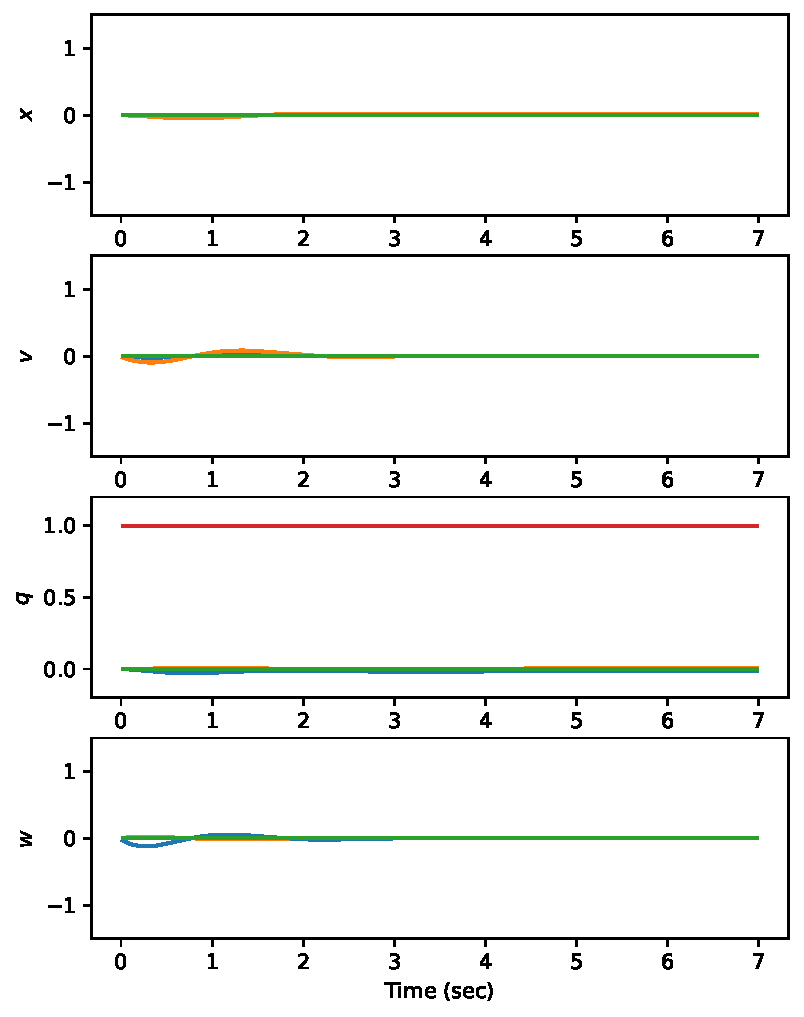
\includegraphics[width=\textwidth]{figures/statehover-oc1.pdf}
 		\caption{orthogonal collocation}
 	\end{subfigure}%
 	 \begin{subfigure}[b]{0.3\textwidth}
 		\centering
 		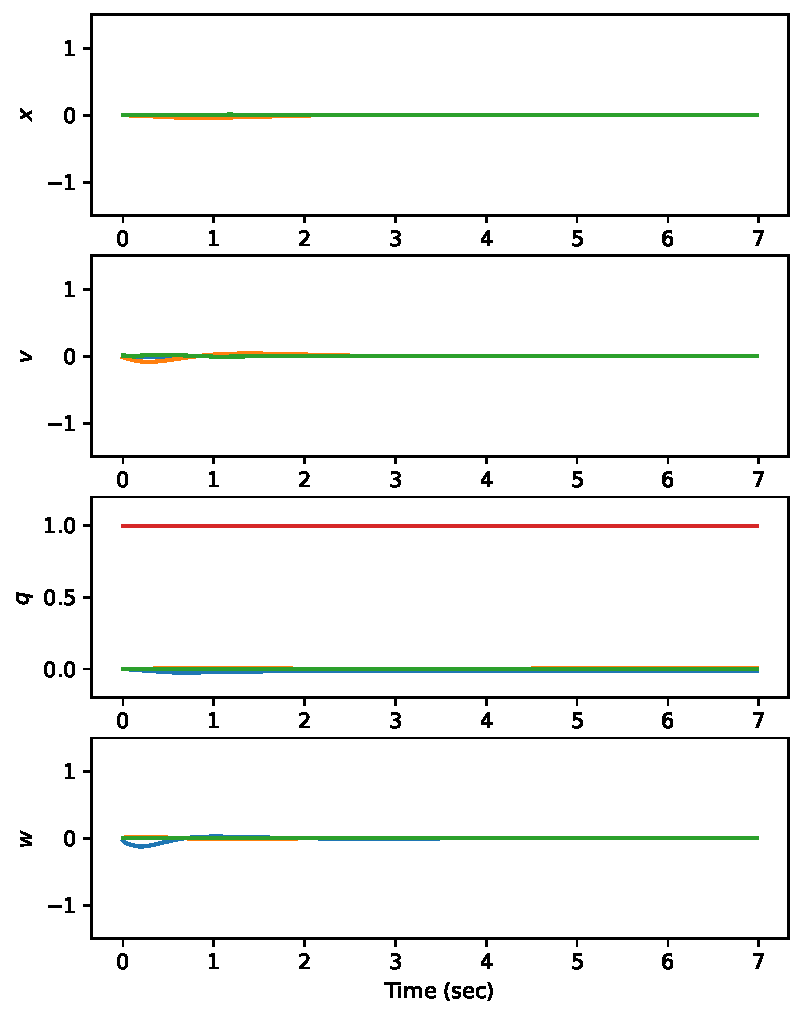
\includegraphics[width=\textwidth]{figures/statehover-cps2.pdf}
 		\caption{Chebyshev pseudospectral}
 	\end{subfigure}
 	\begin{subfigure}[b]{0.3\textwidth}
 		\centering
 		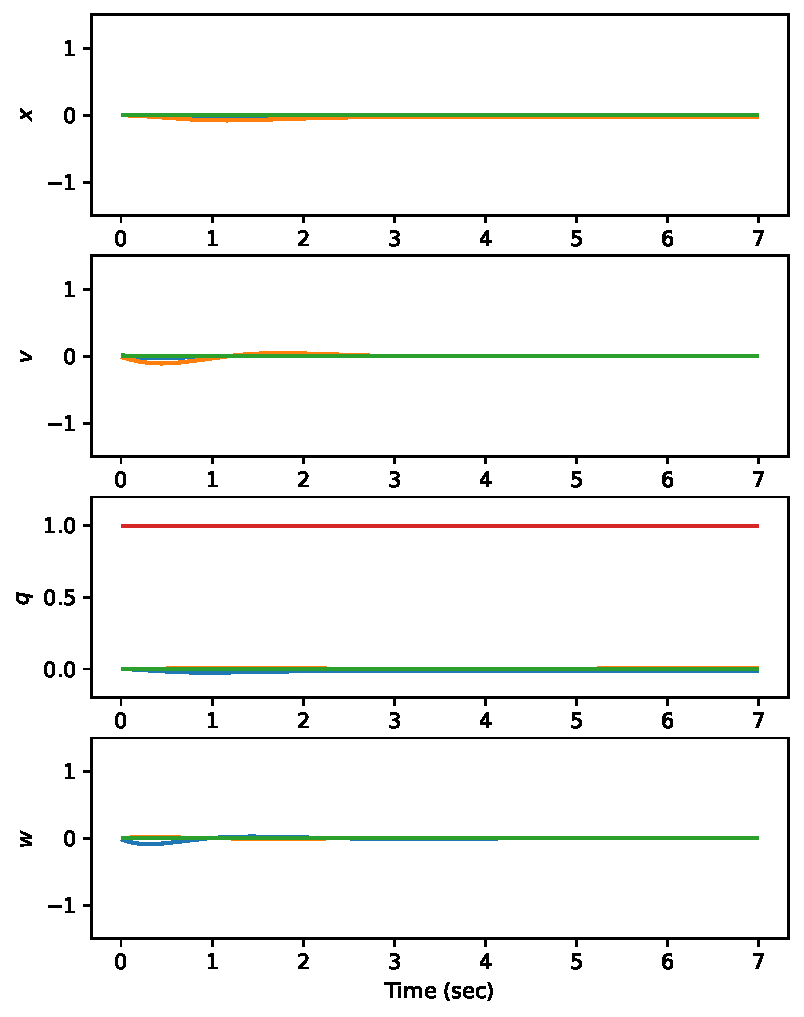
\includegraphics[width=\textwidth]{figures/statehover-ms3.pdf}
 		\caption{multiple shooting}
 	\end{subfigure}
 	\caption{State data on a hover simulation with initial state equal to goal state.}
 	\label{fig:state1}
 \end{figure}
 
 \begin{figure}[H]
 	\centering
 	\begin{subfigure}[b]{0.3\textwidth}
 		\centering
 		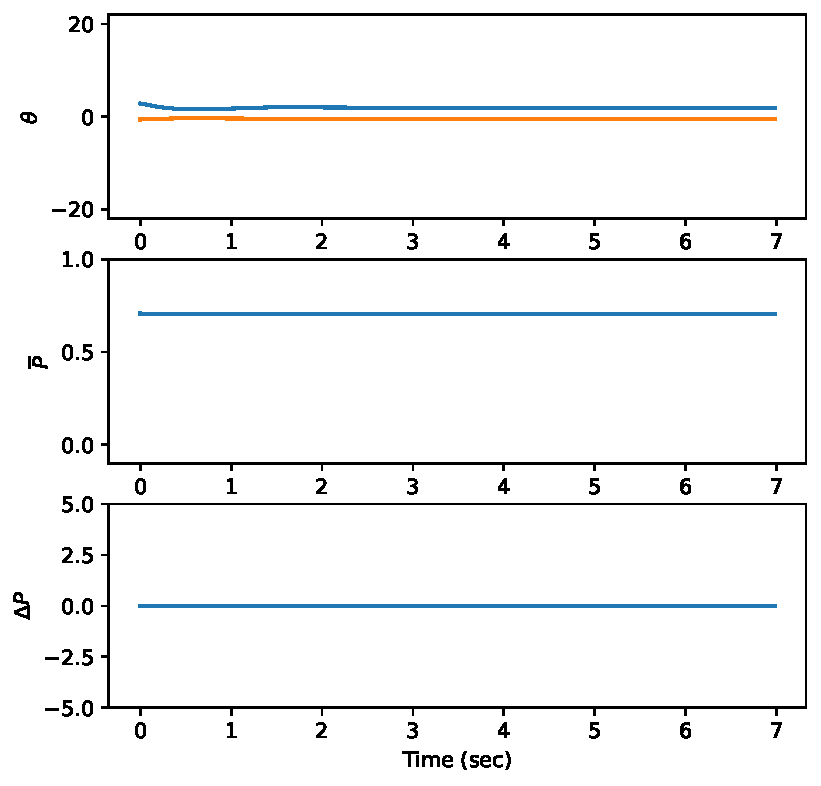
\includegraphics[width=\textwidth]{figures/controlhover-oc4.pdf}
 		\caption{orthogonal collocation}
 	\end{subfigure}%
 	\begin{subfigure}[b]{0.3\textwidth}
 		\centering
 		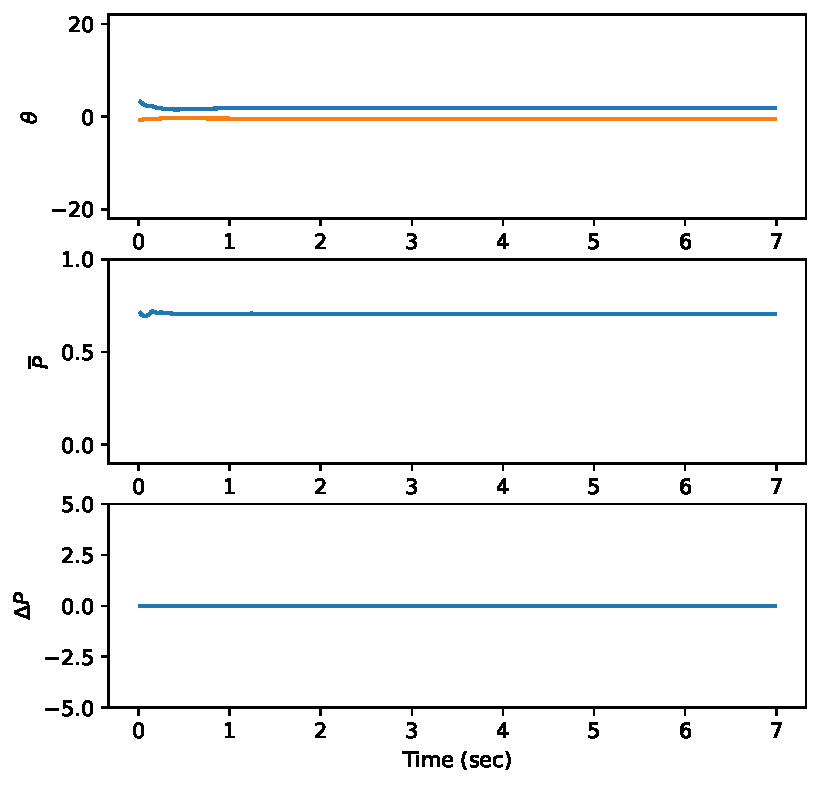
\includegraphics[width=\textwidth]{figures/controlhover-cps5.pdf}
 		\caption{Chebyshev pseudospectral}
 	\end{subfigure}
 	\begin{subfigure}[b]{0.3\textwidth}
		\centering
		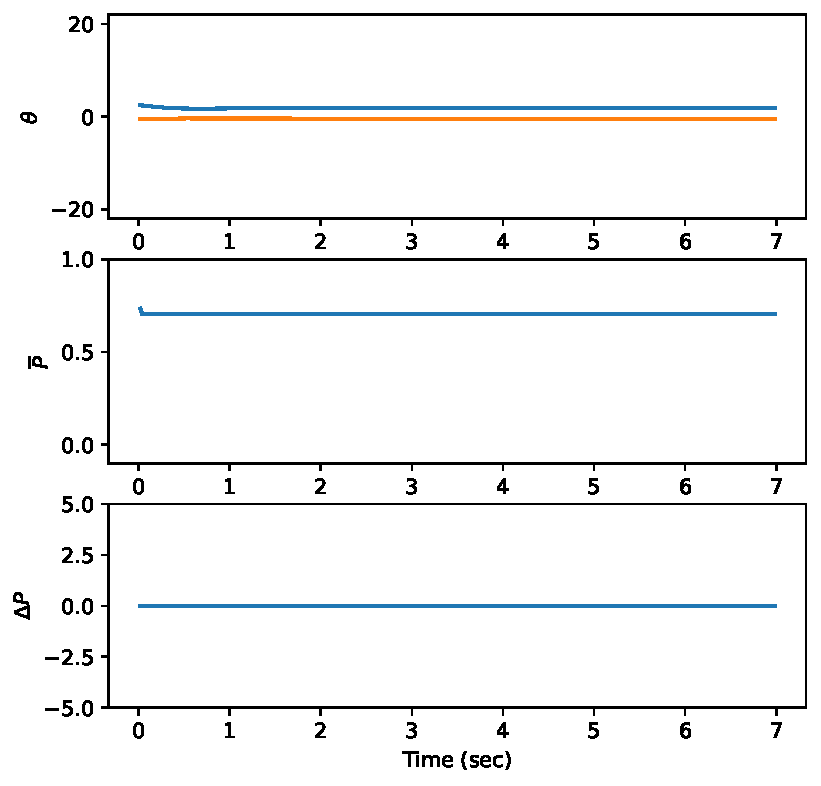
\includegraphics[width=\textwidth]{figures/controlhover-ms6.pdf}
		\caption{multiple shooting}
	\end{subfigure}
 	\caption{Control data on a hover simulation with initial state equal to goal state.}
 	\label{fig:control1}
 \end{figure}
 

 



 %-------------------------------------- SMALL PERTURBATION  ------------------------------------------

 \begin{figure}[H]
	\centering

	\begin{subfigure}[b]{0.3\textwidth}
		\centering
		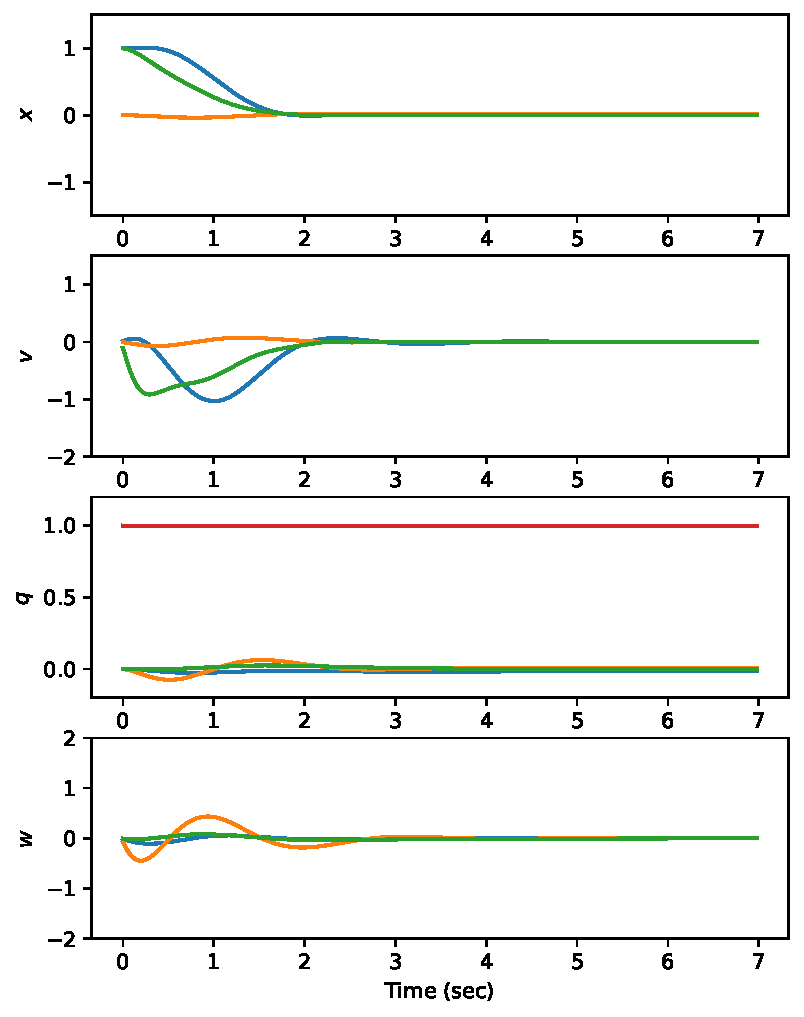
\includegraphics[width=\textwidth]{figures/statemed_perturb-oc1.pdf}
		\caption{orthogonal collocation}
	\end{subfigure}%
	\begin{subfigure}[b]{0.3\textwidth}
		\centering
		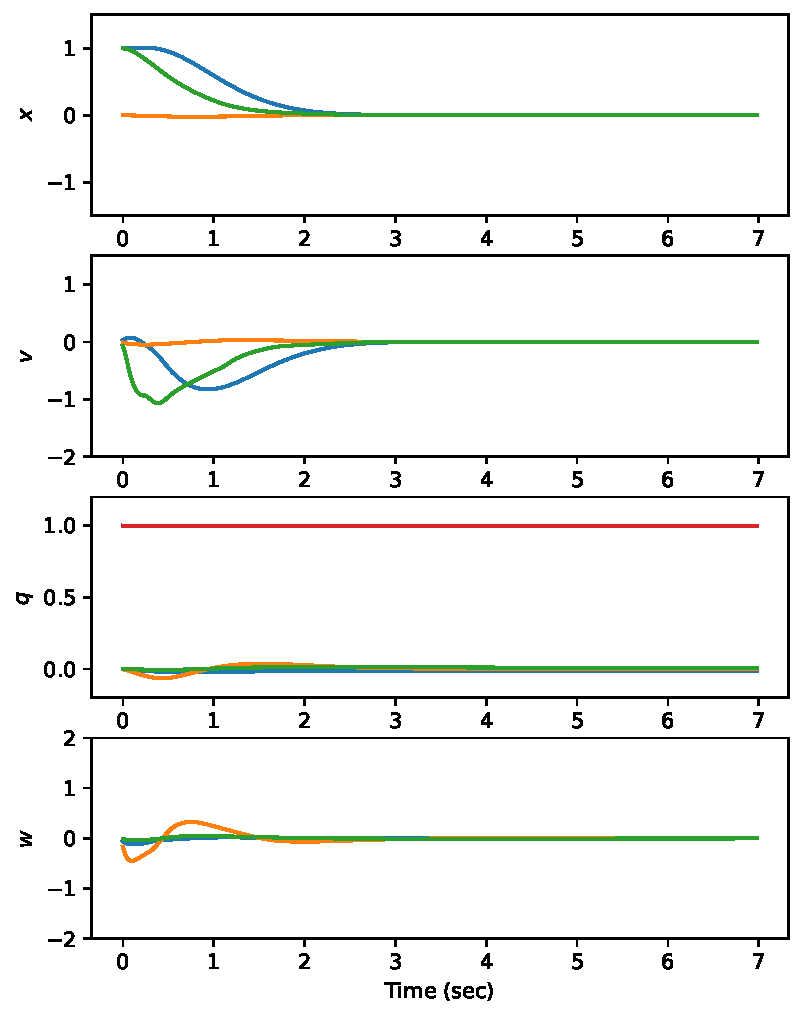
\includegraphics[width=\textwidth]{figures/statemed_perturb-cps2.pdf}
		\caption{Chebyshev pseudospectral}
	\end{subfigure}
	\begin{subfigure}[b]{0.3\textwidth}
		\centering
		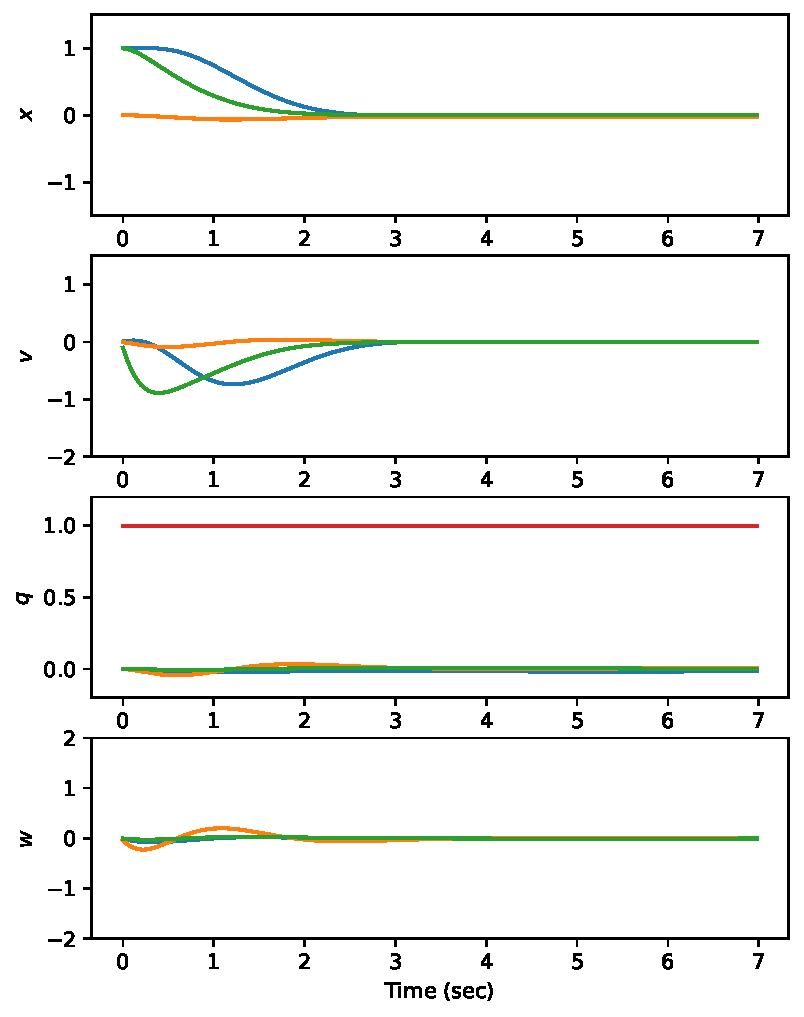
\includegraphics[width=\textwidth]{figures/statemed_perturb-ms3.pdf}
		\caption{multiple shooting}
	\end{subfigure}
	\caption{State data on a simulation with initial position of $[1, 1, 0]$.}
	\label{fig:state2}
\end{figure}

\begin{figure}[H]
	\centering
	\begin{subfigure}[b]{0.3\textwidth}
		\centering
		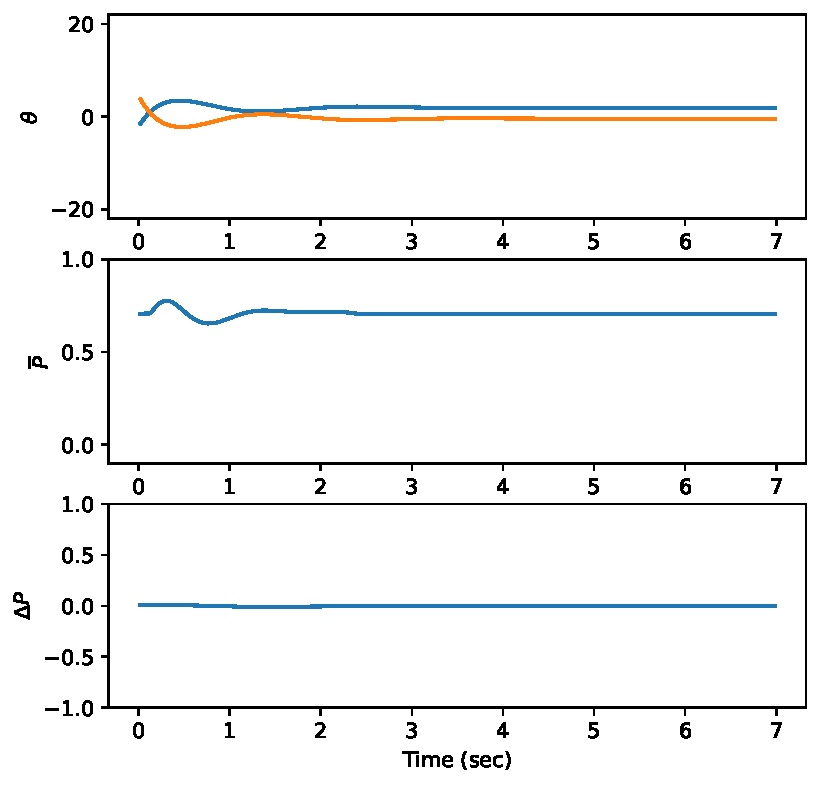
\includegraphics[width=\textwidth]{figures/controlmed_perturb-oc4.pdf}
		\caption{orthogonal collocation}
	\end{subfigure}%
	\begin{subfigure}[b]{0.3\textwidth}
		\centering
		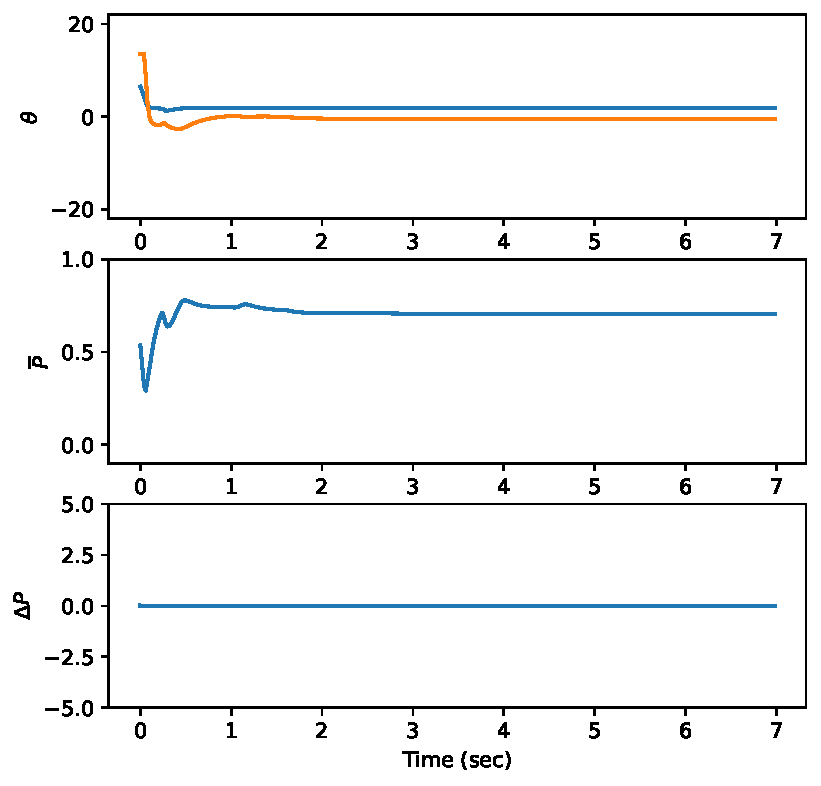
\includegraphics[width=\textwidth]{figures/controlmed_perturb-cps5.pdf}
		\caption{Chebyshev pseudospectral}
	\end{subfigure}
	\begin{subfigure}[b]{0.3\textwidth}
		\centering
		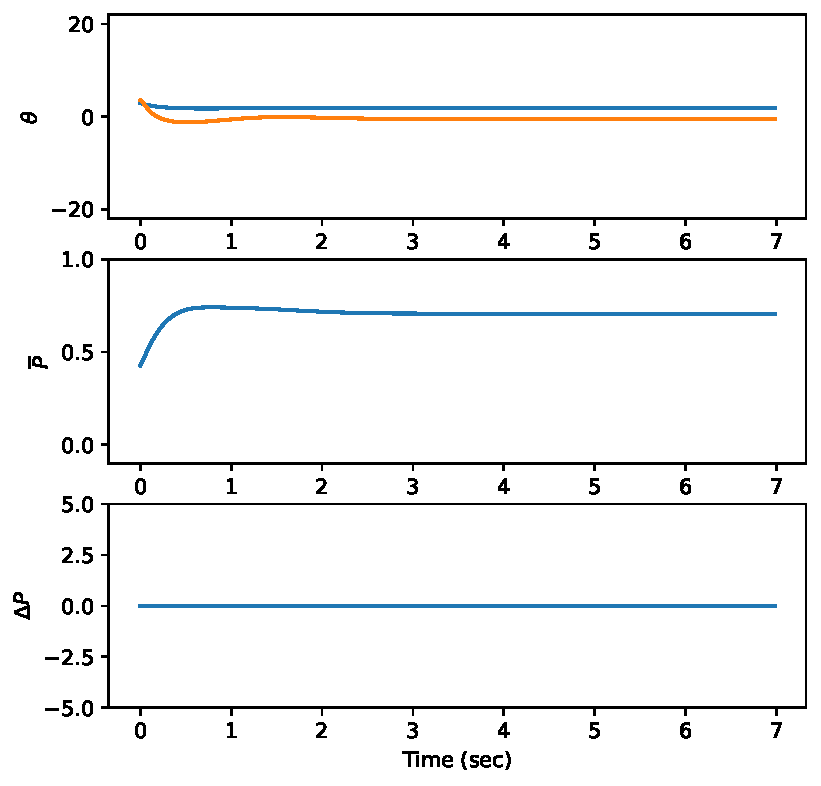
\includegraphics[width=\textwidth]{figures/controlmed_perturb-ms6.pdf}
		\caption{multiple shooting}
	\end{subfigure}
	\caption{Control data on a simulation with initial position of $[1, 1, 0]$.}
	\label{fig:control2}
\end{figure}







 %-------------------------------------- LARGE PERTURBATION  ------------------------------------------


 \begin{figure}[H]
	\centering
	\begin{subfigure}[b]{0.3\textwidth}
		\centering
		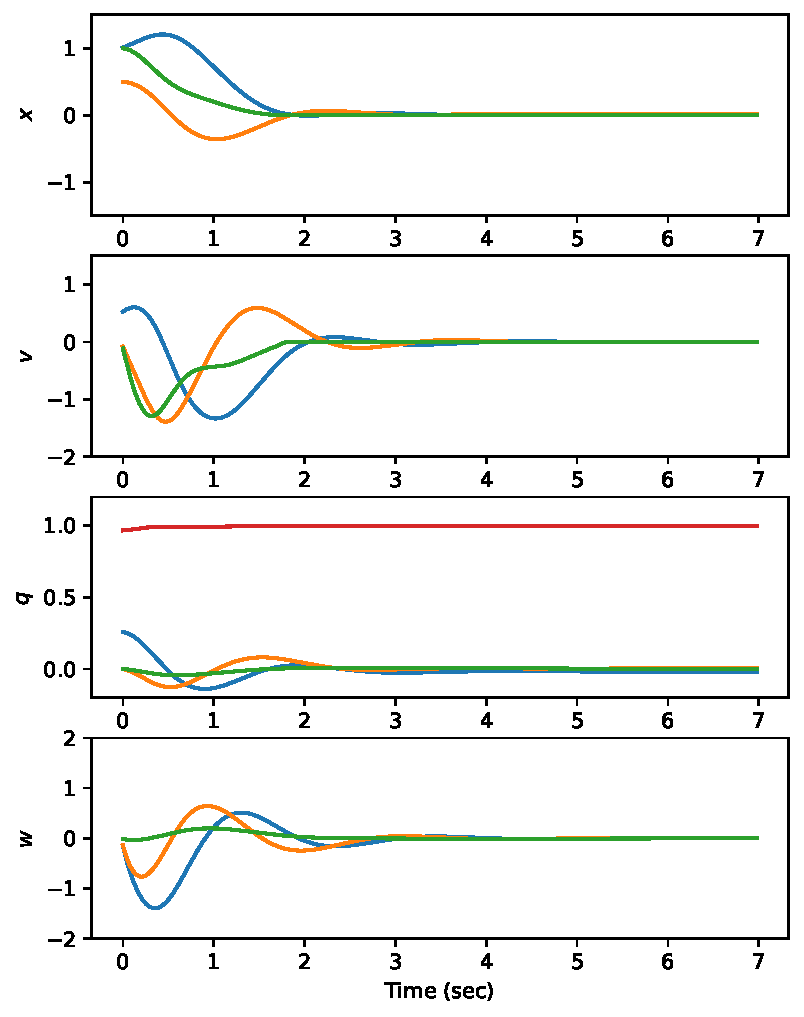
\includegraphics[width=\textwidth]{figures/statebig_perturb-oc1.pdf}
		\caption{orthogonal collocation}
	\end{subfigure}%
	\begin{subfigure}[b]{0.3\textwidth}
		\centering
		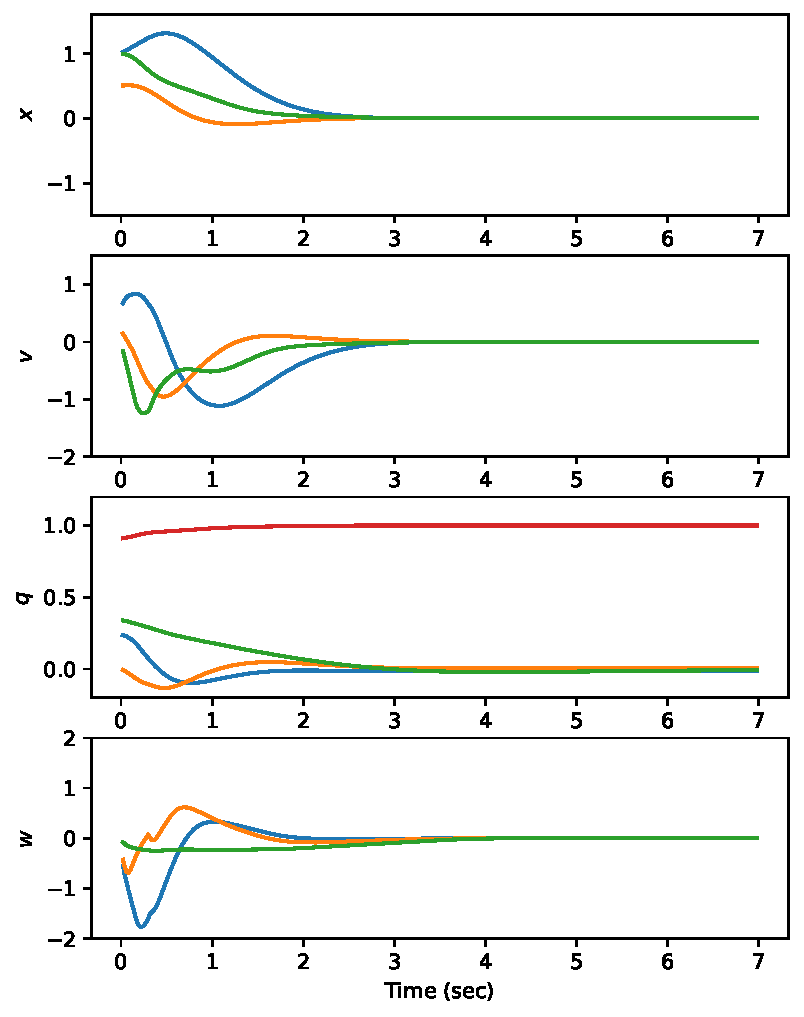
\includegraphics[width=\textwidth]{figures/statebig_perturb-cps2.pdf}
		\caption{Chebyshev pseudospectral}
	\end{subfigure}
	\begin{subfigure}[b]{0.3\textwidth}
		\centering
		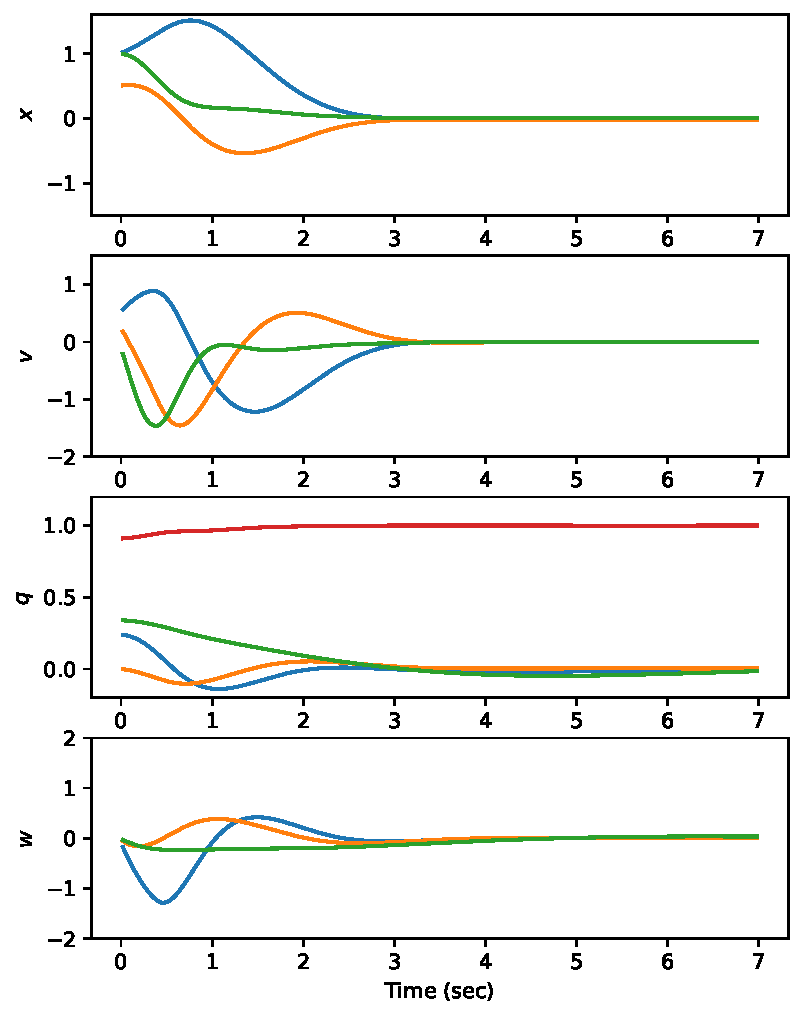
\includegraphics[width=\textwidth]{figures/statebig_perturb-ms3.pdf}
		\caption{multiple shooting}
	\end{subfigure}
	\caption{State data on a simulation with a large starting perturbation.}
	\label{fig:state3}
\end{figure}

\begin{figure}[H]
	\centering
	\begin{subfigure}[b]{0.3\textwidth}
		\centering
		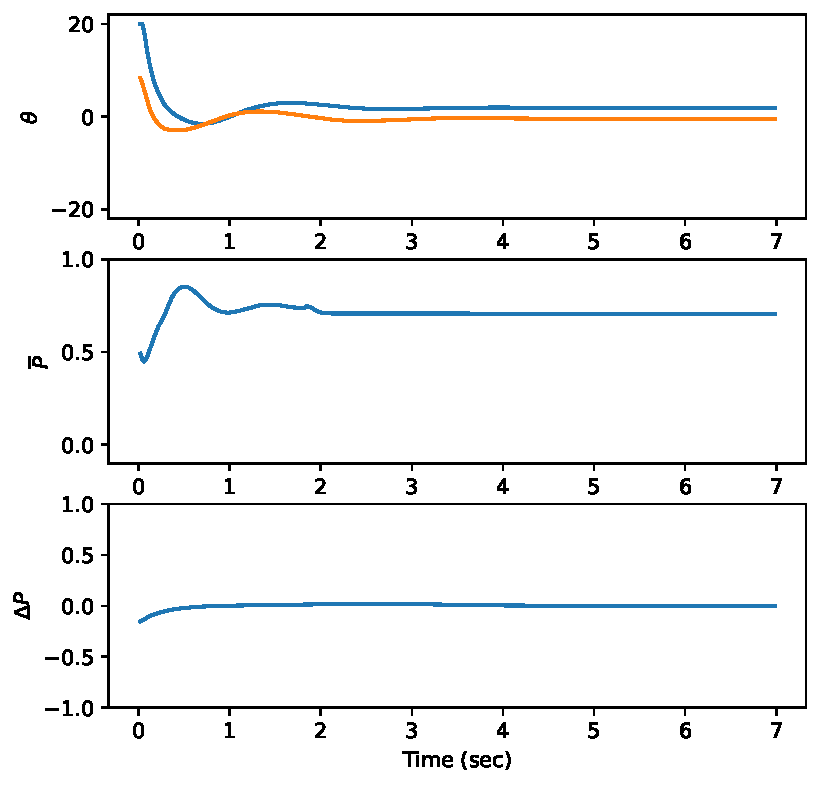
\includegraphics[width=\textwidth]{figures/controlbig_perturb-oc4.pdf}
		\caption{orthogonal collocation}
	\end{subfigure}%
	\begin{subfigure}[b]{0.3\textwidth}
		\centering
		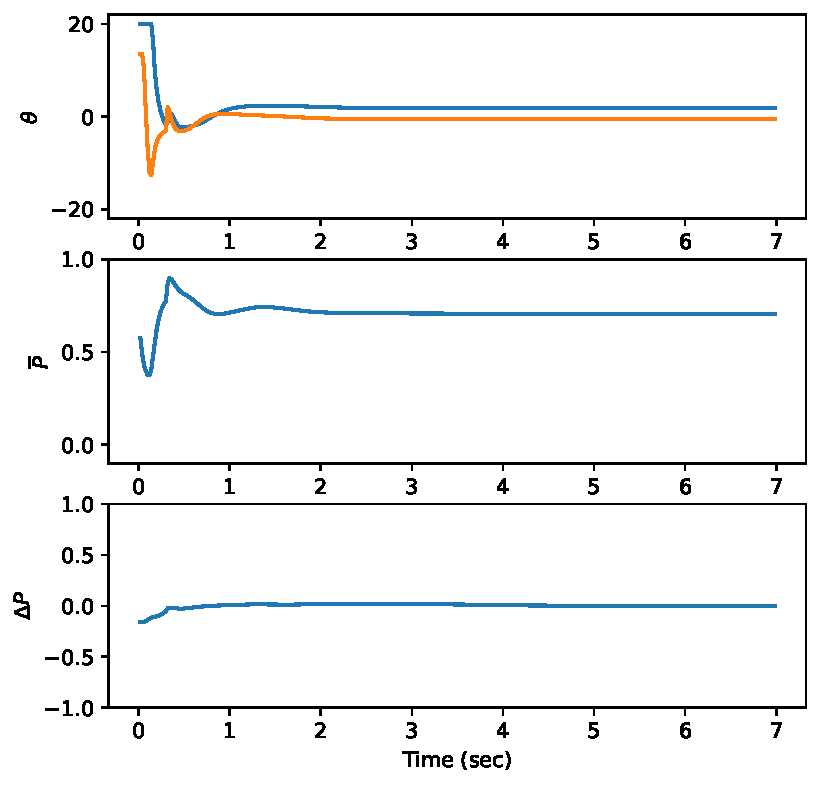
\includegraphics[width=\textwidth]{figures/controlbig_perturb-cps5.pdf}
		\caption{Chebyshev pseudospectral}
	\end{subfigure}
	\begin{subfigure}[b]{0.3\textwidth}
		\centering
		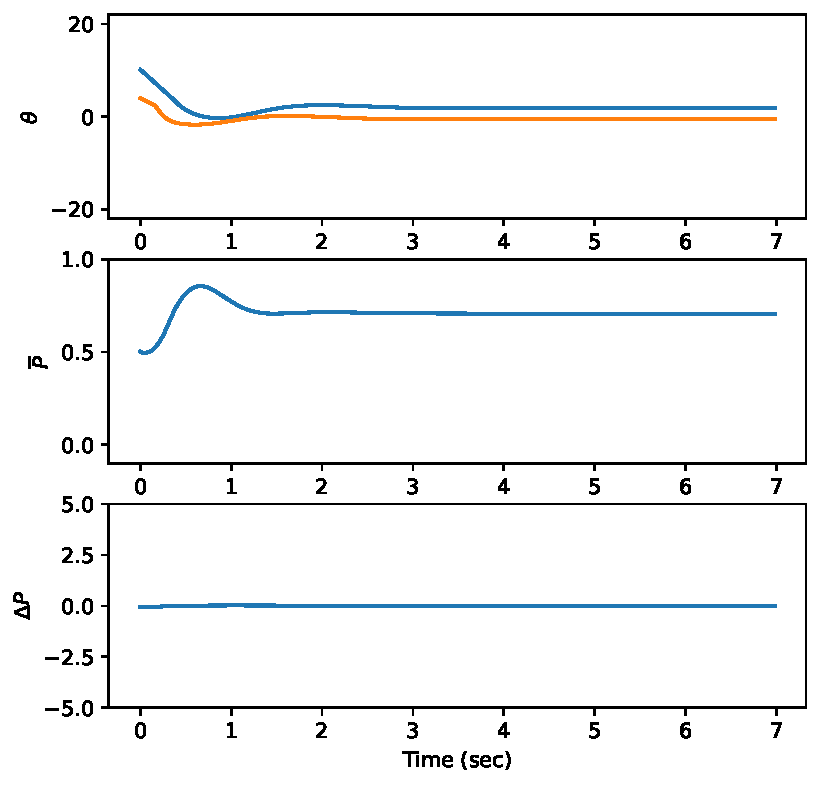
\includegraphics[width=\textwidth]{figures/controlbig_perturb-ms6.pdf}
		\caption{multiple shooting}
	\end{subfigure}

	\caption{Control data on a simulation with a large starting perturbation.}
	\label{fig:control3}
\end{figure}




 \begin{figure}[H]
	\centering
	\begin{subfigure}[b]{0.5\textwidth}
		\centering
	 	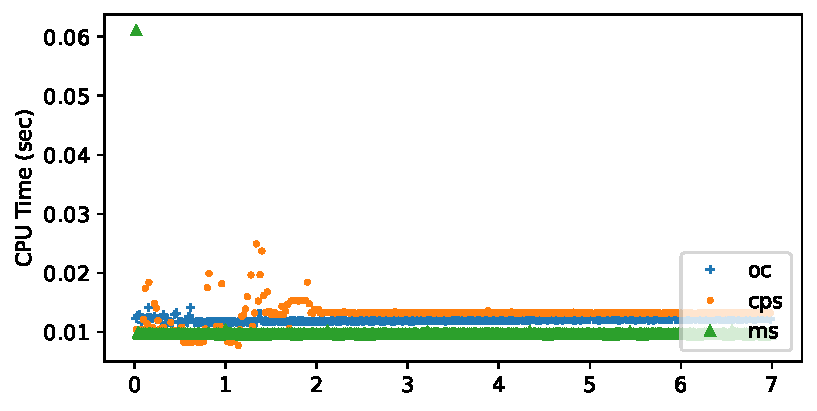
\includegraphics[width=\textwidth]{figures/timehover.pdf}
	\caption{Hover simulation.}
	\end{subfigure}%
	\begin{subfigure}[b]{0.5\textwidth}
		\centering
		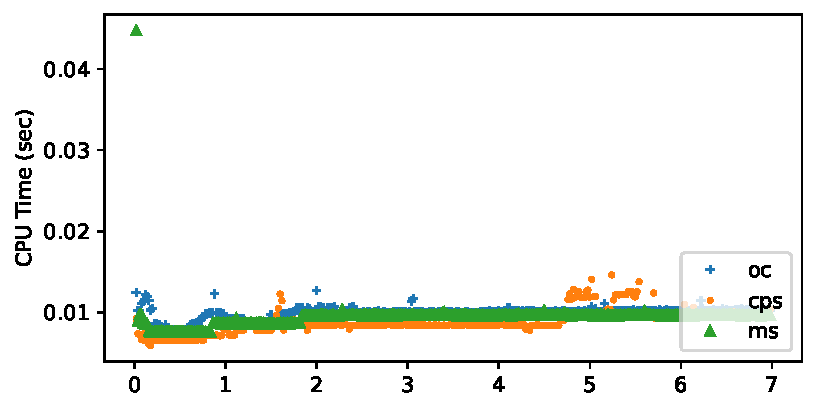
\includegraphics[width=\textwidth]{figures/timemed_perturb.pdf}
	\caption{Initial position of $[1, 1, 0]$.}
	\end{subfigure}
	\begin{subfigure}[b]{0.5\textwidth}
		\centering
		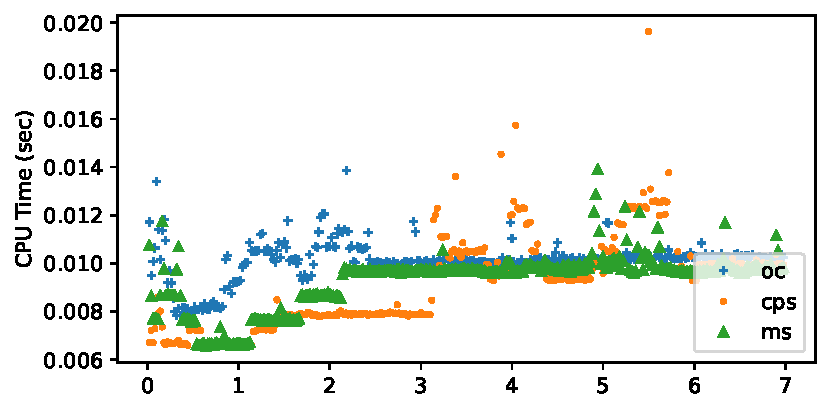
\includegraphics[width=\textwidth]{figures/timebig_perturb.pdf}
		\caption{Large initial perturbation.}
	\end{subfigure}
	\caption{Timing for test cases.}
	\label{fig:timingplots}
\end{figure}


\section{Hardware Validation and Future Work}
\label{hardwarevalidation}
We ran test flights using the NMPC with orthogonal collocation on the drone and achieved successful vertical stabilization and sustained hovering limited only by battery charge. 
Although attitude stabilization was successful, the vehicle exhibited slow oscillatory drift about the vertical axis and did not exhibit the precise position control required.  Supplementary flight videos are available online.\footnote{\url{https://www.youtube.com/watch?v=N2oum2yvaio}}
Analysis of the flight logs showed the presence of a significant constant time delay, which we estimate at approximately 100-200 ms. The cause of the delay is between actuator commands generated on the Raspberry Pi and the observed actuator response. This delay was not present in our simulation environment and substantially degrades closed-loop control performance of the system.
The source of the delay is currently under investigation. We use ROS 2 and Micro XRCE-DDS to communicate between the Raspberry Pi 5 and Pixhawk flight controller. The observed latency might arise from message transport protocols, buffering, scheduling, or mismatched timestamp logic between the Raspberry Pi and Pixhawk. Once the delay has been fixed or compensated for, live flight data can be produced.
Nevertheless, the successful stabilization of the physical platform demonstrates the practical feasibility of implementing real-time NMPC for TVC control on low-cost embedded hardware.

\section{Conclusions}
\label{conclusion}


This paper presents the design of a thrust vector control (TVC) drone platform for investigating nonlinear model predictive control (NMPC) of vertical takeoff and landing (VTOL) systems on low-cost embedded hardware. We experimented with three nonlinear programming (NLP) formulations for the NMPC problem: Runge-Kutta multiple shooting, orthogonal collocation with Gauss-Radau nodes, and Chebyshev pseudospectral collocation.

Our results showed that all three NLP formulations were capable of stabilizing the drone’s nonlinear system with average run times that met our requirement of running at 50 Hz on the Raspberry Pi 5. However, orthogonal collocation provided the most reliable overall performance, keeping all NLP solution times within the allotted $0.02s$ time interval, producing smooth convergent trajectories and avoiding NLP solver failures. In addition, orthogonal collocation was the easiest to implement due to the availability of the {\dompc} library. The Chebyshev pseudospectral collocation method had less consistent timing behavior and slightly irregular control trajectories. 
Multiple shooting demonstrated good trajectory quality and computational performance but had occasional NLP solver failures and timing spikes.


We deployed the NMPC controller using orthogonal collocation on the physical drone. Initial experiments showed successful stabilization when hovering, but flight data analysis exhibited significant actuator-response latency possibly caused by communication protocols in the messaging pipeline. This timing lag must be fixed or accommodated before precise position control can be attained.


\bibliography{references.bib}
\end{document}

